\documentclass[10pt,a4paper]{article}
\usepackage[latin1]{inputenc}
\usepackage{amsmath}
\usepackage{microtype}
\usepackage[none]{hyphenat}
\usepackage{verbatim}
\usepackage{amsfonts}
\usepackage{amssymb}
\usepackage{enumitem}
\renewcommand{\familydefault}{\sfdefault}
\usepackage{mathpazo}
\renewcommand{\rmdefault}{put}
\usepackage{enumitem}
\usepackage[dvipsnames,svgnames]{xcolor}
\usepackage{tkz-euclide}
\usetkzobj{all}
\usepackage{graphicx}
\usepackage{tikz} 	
\usepackage{pgfplots}
\usepackage{adjustbox}
\usepackage{multicol}
\usepackage{lipsum}
\usepackage[left=0.7cm,right=0.7cm,top=1cm,bottom=1.5cm]{geometry}
\usepackage{cancel} \usepackage{xcolor}
\usepackage{tcolorbox}

\pgfplotsset{every x tick label/.append style={font=\tiny, yshift=0.5ex}}
\pgfplotsset{every y tick label/.append style={font=\tiny, xshift=0.5ex}}

\usetikzlibrary{decorations.pathmorphing,patterns}
\usetikzlibrary{decorations.pathreplacing,calc}
 \newcommand\coret[2][red]{\renewcommand\CancelColor{\color{#1}}\cancel{#2}}
\SetLabelAlign{Center}{\hfil\makebox[1.0em]{#1}\hfil}

%%_------= solusi


% Set this =0 to hide, =1 to show

% Set this =0 to hide, =1 to show
\newtcolorbox{mybox}[1][] { colframe = blue!10, colback = blue!3,boxsep=0pt,left=0.2em, coltitle = blue!20!black, title = \textbf{jawab}, #1, } 

%---------- kunci (jika 1 ) muncul
\def\tampilkunci{1}
\newcommand{\hide}[1]{\ifnum\tampilkunci=1
%
\begin{mybox}
 #1
\end{mybox}
%
\vspace{\baselineskip}\fi}



\newcommand*\cicled[1]{\tikz[baseline=(char.base)]{\node[white, shape=circle, fill=red!80,draw,inner sep=0.5pt](char){#1};}}

\newcommand*\kunci[1]{\ifnum\tampilkunci=1
%
\tikz[baseline=(char.base)]{\node[red, shape=circle,draw,inner sep=0.5pt,xshift=2pt](char){#1};}\stepcounter{enumii}
\fi\ifnum\tampilkunci=0
%
\hspace{3pt}#1\stepcounter{enumii}
%
\fi}

\newcommand*\silang[1]{\tikz[baseline=(char.base)]{
\draw[red,thick](-0.2,-0.20)--(0.2,0.2);
\draw[red,thick](-0.2,0.20)--(0.2,-0.2);
\node[black](char){#1};
}}

\newcommand*\centang[1]{\tikz[baseline=(char.base)]{
\draw[red, very thick](-0.2,0.1)--(-0.1,0)--(0.2,0.3);
\node(char){#1};
}}

\newcommand*\merah[1]{
\textcolor{red}{#1}}
\newcommand*\pilgan[1]{
\begin{enumerate}[label=\Alph*., itemsep=0pt,topsep=0pt,leftmargin=*,align=Center] #1 
\end{enumerate}}
\newcommand*\pernyataan[1]{
\begin{enumerate}[label=(\arabic*), itemsep=0pt,topsep=0pt,leftmargin=*] #1 
\end{enumerate}}

\newcommand{\pilgani}[1]{                            \vspace{-0.3cm}\begin{multicols}{2}
 \begin{enumerate}[label=\Alph*., itemsep=0pt,topsep=0pt,leftmargin=*,align=Center]#1                     \end{enumerate}
 \phantom{ini cuma sapi, wedus, dan ayam}
 \end{multicols}}


\begin{document}

\begin{multicols*}{2}

\begin{enumerate}




\end{enumerate}
    
                                                                                                                                                  
                                                                                                                                                   
                                                                                                                                                   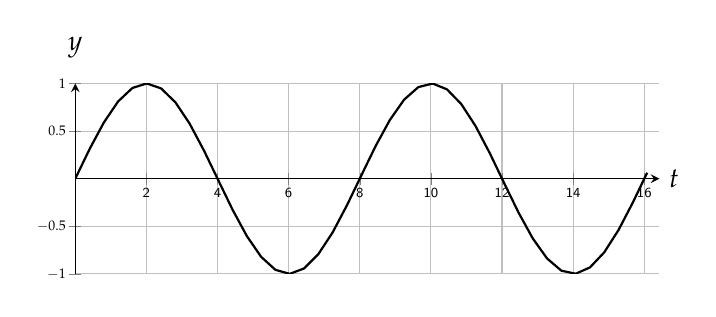
\begin{tikzpicture}
\begin{axis}[
    axis x line=center,
    ylabel={$y$},
    xlabel={$t$}, 
    axis y line=middle,
    every axis x label/.style={at={(current axis.right of origin)},anchor=west},
    every axis y label/.style={at={(current axis.north west)},above=2mm}, 
    xtick={0,1.5708,3.14159,...,14},
    xticklabels={0,2,...,16},
      xmin=.0, xmax=12.90,
    domain=0:4.02*pi, width=9cm,height=4cm,
    samples=41,grid]
\addplot[thick, black, no marks] {sin(deg(x))};
\end{axis}
\end{tikzpicture}



                                                                                                                                                   


\end{enumerate}

\end{multicols*}


 \end{document}






